\documentclass[]{article}

\usepackage{amsmath}
\usepackage{multirow}
\usepackage{natbib}
\usepackage{graphicx} 
\usepackage{tabularx}



\begin{document}

\title{Anomalous Transport and Ergodicity in Chaotic Point-Vortex Systems: A Comparison with Lévy Walks}

\author{Denario}
\date{Anthropic, Gemini \& OpenAI servers. Planet Earth.}

\maketitle
\begin{abstract}
The transport of passive tracers in two-dimensional chaotic flows is often characterized by anomalous superdiffusion, yet whether these complex Hamiltonian systems can be effectively described by canonical stochastic models like Lévy walks remains an open question. We address this by directly comparing numerical simulations of tracer trajectories in point-vortex systems of varying chaoticity, controlled by the number of vortices $N$, with a benchmark dataset of Lévy walks. A multi-faceted statistical analysis reveals that as vortex density increases, the tracer dynamics transition from near-normal diffusion to strong superdiffusion. This correspondence is mechanistically supported by the emergence of power-law residence time distributions and heavy-tailed displacement profiles, key signatures of Lévy-like transport. Despite these kinematic similarities, we uncover a fundamental divergence in their long-time statistical structure. We demonstrate that the vortex system becomes progressively more ergodic as superdiffusion strengthens with increasing $N$, a trend that is diametrically opposed to the increasing non-ergodicity of superdiffusive Lévy walks. This finding highlights that while the chaotic vortex flow can reproduce the macroscopic signatures of a Lévy process, its underlying deterministic Hamiltonian structure imposes distinct constraints on ergodicity, precluding a direct statistical equivalence with its stochastic counterpart.
\end{abstract}








\section{Introduction}
\label{sec:intro}
The transport of passive particles in chaotic fluid flows is a fundamental problem in non-equilibrium statistical mechanics, with applications ranging from pollutant dispersal in the atmosphere and oceans to mixing processes in planetary interiors. In such systems, the intricate, deterministic motion of the fluid often drives particle trajectories that deviate strongly from classical Brownian motion. A common manifestation of this is anomalous superdiffusion, where the mean squared displacement grows faster than linearly with time, $\langle \Delta r^2(t) \rangle \propto t^\alpha$, with an anomalous exponent $\alpha > 1$. This behavior signals the presence of long-range correlations in the particle's velocity, posing a significant challenge to theoretical modeling: can the complex dynamics generated by a deterministic system be effectively captured by a simpler, canonical stochastic process?

The Lévy walk model has emerged as a leading theoretical framework for describing superdiffusion in physical systems. It conceptualizes a particle performing a sequence of ballistic flights, where the duration of each flight is drawn from a heavy-tailed, power-law distribution. This construction naturally gives rise to superdiffusive scaling while respecting a finite particle velocity, making it a physically plausible model for transport phenomena. The apparent success of Lévy walks in reproducing the macroscopic scaling observed in various chaotic systems raises a critical question: does this kinematic similarity imply a deeper statistical equivalence? It remains an open problem whether the full statistical structure of transport in a deterministic, chaotic Hamiltonian flow can be faithfully mapped onto a purely stochastic process like a Lévy walk.

To address this question, we conduct a direct and systematic comparison between tracer transport in a chaotic point-vortex system and a benchmark Lévy walk process. The two-dimensional point-vortex flow serves as an ideal model system; it is a conservative Hamiltonian flow that represents a foundational model for ideal 2D turbulence, and its degree of chaoticity can be precisely controlled by varying the number of vortices, $N$. We numerically simulate the trajectories of passive tracers advected by these flows for systems with increasing vortex density and compare their statistical properties against a comprehensive dataset of Lévy walk trajectories. Our analysis employs a suite of diagnostics, including the scaling of the mean squared displacement, velocity autocorrelation functions, residence time distributions in low-velocity regions, and the evolution of displacement probability distributions.

Our investigation first confirms that as the vortex density increases, the point-vortex system kinematically mimics a Lévy process. The transport transitions from near-normal diffusion to strong superdiffusion, accompanied by the emergence of power-law residence times and heavy-tailed displacement profiles, which are hallmark signatures of Lévy-like dynamics. However, the central contribution of this work is to move beyond these kinematic measures and probe the ergodicity of the underlying statistical ensembles. We uncover a fundamental divergence between the two systems. As the superdiffusive behavior in the vortex system strengthens with increasing $N$, the system becomes progressively more ergodic. This trend is in stark opposition to the behavior of Lévy walks, which become increasingly non-ergodic as their superdiffusive character intensifies. This finding reveals that despite reproducing key macroscopic signatures of a Lévy process, the deterministic and Hamiltonian constraints of the vortex flow impose a distinct statistical structure, precluding a complete equivalence with its stochastic counterpart and highlighting that kinematic similarity alone is an insufficient criterion for model validation.

\section{Methods}
\label{sec:methods}
\subsection{Numerical models}

We conduct a comparative analysis between two distinct dynamical systems: a deterministic Hamiltonian point-vortex flow and a canonical stochastic Lévy walk model.

\subsubsection{Point-vortex system}
The motion of a passive tracer at position $\mathbf{r} = (x, y)$ is governed by the advection in a two-dimensional velocity field $\mathbf{u}(\mathbf{r}, t)$ generated by $N$ point vortices. The velocity field is the superposition of the fields induced by each vortex:
\begin{equation}
\dot{\mathbf{r}} = \mathbf{u}(\mathbf{r}, t) = \sum_{k=1}^{N} \frac{\Gamma_k}{2\pi} \frac{\hat{\mathbf{z}} \times (\mathbf{r} - \mathbf{r}_k(t))}{|\mathbf{r} - \mathbf{r}_k(t)|^2}
\end{equation}
where $\mathbf{r}_k(t)$ and $\Gamma_k$ are the position and circulation of the $k$-th vortex, respectively, and $\hat{\mathbf{z}}$ is the unit vector normal to the plane. The vortices themselves are advected by the same velocity field, creating a self-consistent, time-dependent chaotic flow. The system is Hamiltonian, and its degree of chaoticity is controlled by the number of vortices, $N$.

\subsubsection{Lévy walk model}
As a benchmark stochastic process, we employ a standard Lévy walk model. A particle moves with a constant speed $v_0$ in a straight line for a duration $\tau$. At the end of each flight, a new direction is chosen uniformly at random from $[0, 2\pi)$. The flight times $\tau$ are drawn from a heavy-tailed probability distribution:
\begin{equation}
P(\tau) \sim \tau^{-\beta-1}
\end{equation}
for $\tau \ge \tau_{min}$, where $\beta$ is the characteristic exponent that controls the transport dynamics. For $1 < \beta < 2$, the model produces superdiffusion with a theoretical mean squared displacement exponent of $\alpha = 3 - \beta$. For $\beta > 2$, the mean flight time is finite, leading to normal diffusion with $\alpha=1$.

\subsection{Simulation datasets}

The analysis is based on two primary datasets of simulated trajectories.

For the point-vortex system, we generated trajectories for four configurations with an increasing number of vortices: $N=5, 10, 20,$ and $40$. For each configuration, the vortex circulations $\Gamma_k$ were drawn from a standard normal distribution, and their initial positions were sampled uniformly within a square domain. We then simulated the trajectories of 5 passive tracers for each of the four vortex configurations. Each trajectory was integrated for a total duration of 24.75 s with a time step of 0.05 s. All analyses were performed on these noise-free tracer trajectories.

For the Lévy walk model, we generated a benchmark dataset comprising large ensembles of trajectories for four classes of the tail exponent: $\beta = 1.2, 1.5, 1.8,$ and $2.5$. These values were chosen to span the range from strong superdiffusion ($\alpha=1.8$) to normal diffusion ($\alpha=1.0$). All walkers were simulated with a constant speed of $v_0 = 1.0$ m/s.

\subsection{Statistical analysis}

We employed a suite of statistical tools to characterize and compare the transport properties of both systems.

\subsubsection{Mean squared displacement}
The primary measure of transport is the ensemble-averaged mean squared displacement (MSD), calculated as:
\begin{equation}
\langle \Delta r^2(\Delta t) \rangle = \langle |\mathbf{r}(t+\Delta t) - \mathbf{r}(t)|^2 \rangle
\end{equation}
where the average $\langle \cdot \rangle$ is taken over all possible start times $t$ and all trajectories within a given ensemble. The anomalous diffusion exponent, $\alpha$, was determined by fitting a power law, $\langle \Delta r^2(\Delta t) \rangle \propto (\Delta t)^\alpha$, to the MSD curves on a log-log scale. The fit was performed over a range of lag times from 10\% to 60\% of the maximum trajectory duration to exclude initial ballistic effects and late-time statistical noise.

\subsubsection{Velocity autocorrelation function}
To probe the temporal memory of the dynamics, we computed the normalized velocity autocorrelation function (VACF):
\begin{equation}
C_v(\Delta t) = \frac{\langle \mathbf{v}(t) \cdot \mathbf{v}(t+\Delta t) \rangle}{\langle |\mathbf{v}(t)|^2 \rangle}
\end{equation}
Tracer velocities $\mathbf{v}(t)$ were calculated from the position data using a central finite difference scheme. The VACF measures the persistence of velocity, with its decay rate indicating the characteristic decorrelation time of the flow as experienced by the tracer.

\subsubsection{Residence time distribution}
To mechanistically investigate the origins of anomalous transport, we analyzed the statistics of trapping events. A tracer was defined as being in a "trapped" state whenever its instantaneous speed fell below the 25th percentile of the pooled speed distribution for its respective N-vortex configuration. We measured the duration, $\tau_{res}$, of each continuous trapping event and constructed the probability distribution $P(\tau_{res})$. The tail of this distribution was fitted with a power law, $P(\tau_{res}) \sim \tau_{res}^{-\gamma}$, to identify Lévy-like trapping behavior.

\subsubsection{Displacement probability density functions}
We examined the evolution of the one-dimensional displacement probability density function (PDF), $P(\Delta x)$, for various lag times $\Delta t$, where $\Delta x(t, \Delta t) = x(t+\Delta t) - x(t)$. The shape of these distributions provides insight into the nature of the underlying random process. For the most superdiffusive cases (N=40 vortex system and $\beta=1.5$ Lévy walk), the empirical PDFs at long lag times were compared to both Gaussian and symmetric Lévy-stable distributions to test for convergence to a non-Gaussian attractor.

\subsubsection{Ergodicity analysis}
To quantify the statistical heterogeneity across trajectories, we measured the ergodicity-breaking (EB) parameter. First, we computed the time-averaged MSD (TAMSD) for each individual trajectory $i$:
\begin{equation}
\overline{\delta_i^2(\Delta t)} = \frac{1}{T-\Delta t} \int_0^{T-\Delta t} |\mathbf{r}_i(t'+\Delta t) - \mathbf{r}_i(t')|^2 dt'
\end{equation}
where $T$ is the total observation time. The EB parameter is then defined as the normalized variance of the TAMSDs across the ensemble of trajectories:
\begin{equation}
EB(\Delta t) = \frac{\text{Var}[\overline{\delta^2(\Delta t)}]}{(\text{Mean}[\overline{\delta^2(\Delta t)}])^2} = \frac{\langle (\overline{\delta^2})^2 \rangle - \langle \overline{\delta^2} \rangle^2}{\langle \overline{\delta^2} \rangle^2}
\end{equation}
An EB value of zero signifies perfect ergodicity, while a sustained positive value indicates that individual trajectories exhibit statistically distinct diffusive properties. We characterized the degree of non-ergodicity by calculating a plateau value, defined as the mean of $EB(\Delta t)$ over the final 20\% of the available lag times.

\section{Results}
\label{sec:results}
Our analysis systematically compares the statistical properties of tracer transport in a chaotic point-vortex system with a canonical Lévy walk model. We begin with a qualitative overview of the trajectory morphologies and then proceed to a quantitative analysis of transport scaling, its underlying mechanisms, and the ergodicity of the ensembles.

\subsection{Tracer trajectory morphology}

A visual inspection of representative tracer trajectories reveals a strong dependence of the transport characteristics on the number of vortices, $N$, as shown in Figure \ref{fig:trajectories}. For a low vortex count ($N=5$), the tracer path is compact and exhibits quasi-periodic, looping structures. This indicates that the dynamics are weakly chaotic, and the tracer remains confined within the influence of a few dominant vortices, failing to explore the full spatial domain within the simulation time.

As $N$ increases, the trajectories become progressively more erratic and space-filling. The $N=20$ case shows intermittent behavior, with periods of local trapping punctuated by long-range excursions. This morphology intensifies in the $N=40$ system, where the trajectory consists of numerous long, nearly ballistic flights connecting distinct, tortuous regions. This visual evidence suggests a transition towards a Lévy-like transport regime at high vortex densities.

A comparison with the benchmark Lévy walk trajectories (bottom row of Figure \ref{fig:trajectories}) reinforces this observation. The strongly superdiffusive Lévy walk ($\beta=1.5$) produces a trajectory that is morphologically similar to the $N=40$ vortex case. Conversely, the normal-diffusive Lévy walk ($\beta=2.5$) results in a compact, tortuous path reminiscent of the weakly chaotic $N=5$ vortex system. A key distinction remains: the "flights" in the vortex system are continuously curved due to the persistent influence of the velocity field, unlike the perfectly straight flights of the idealized Lévy walk.

\begin{figure}[t]
    \centering
    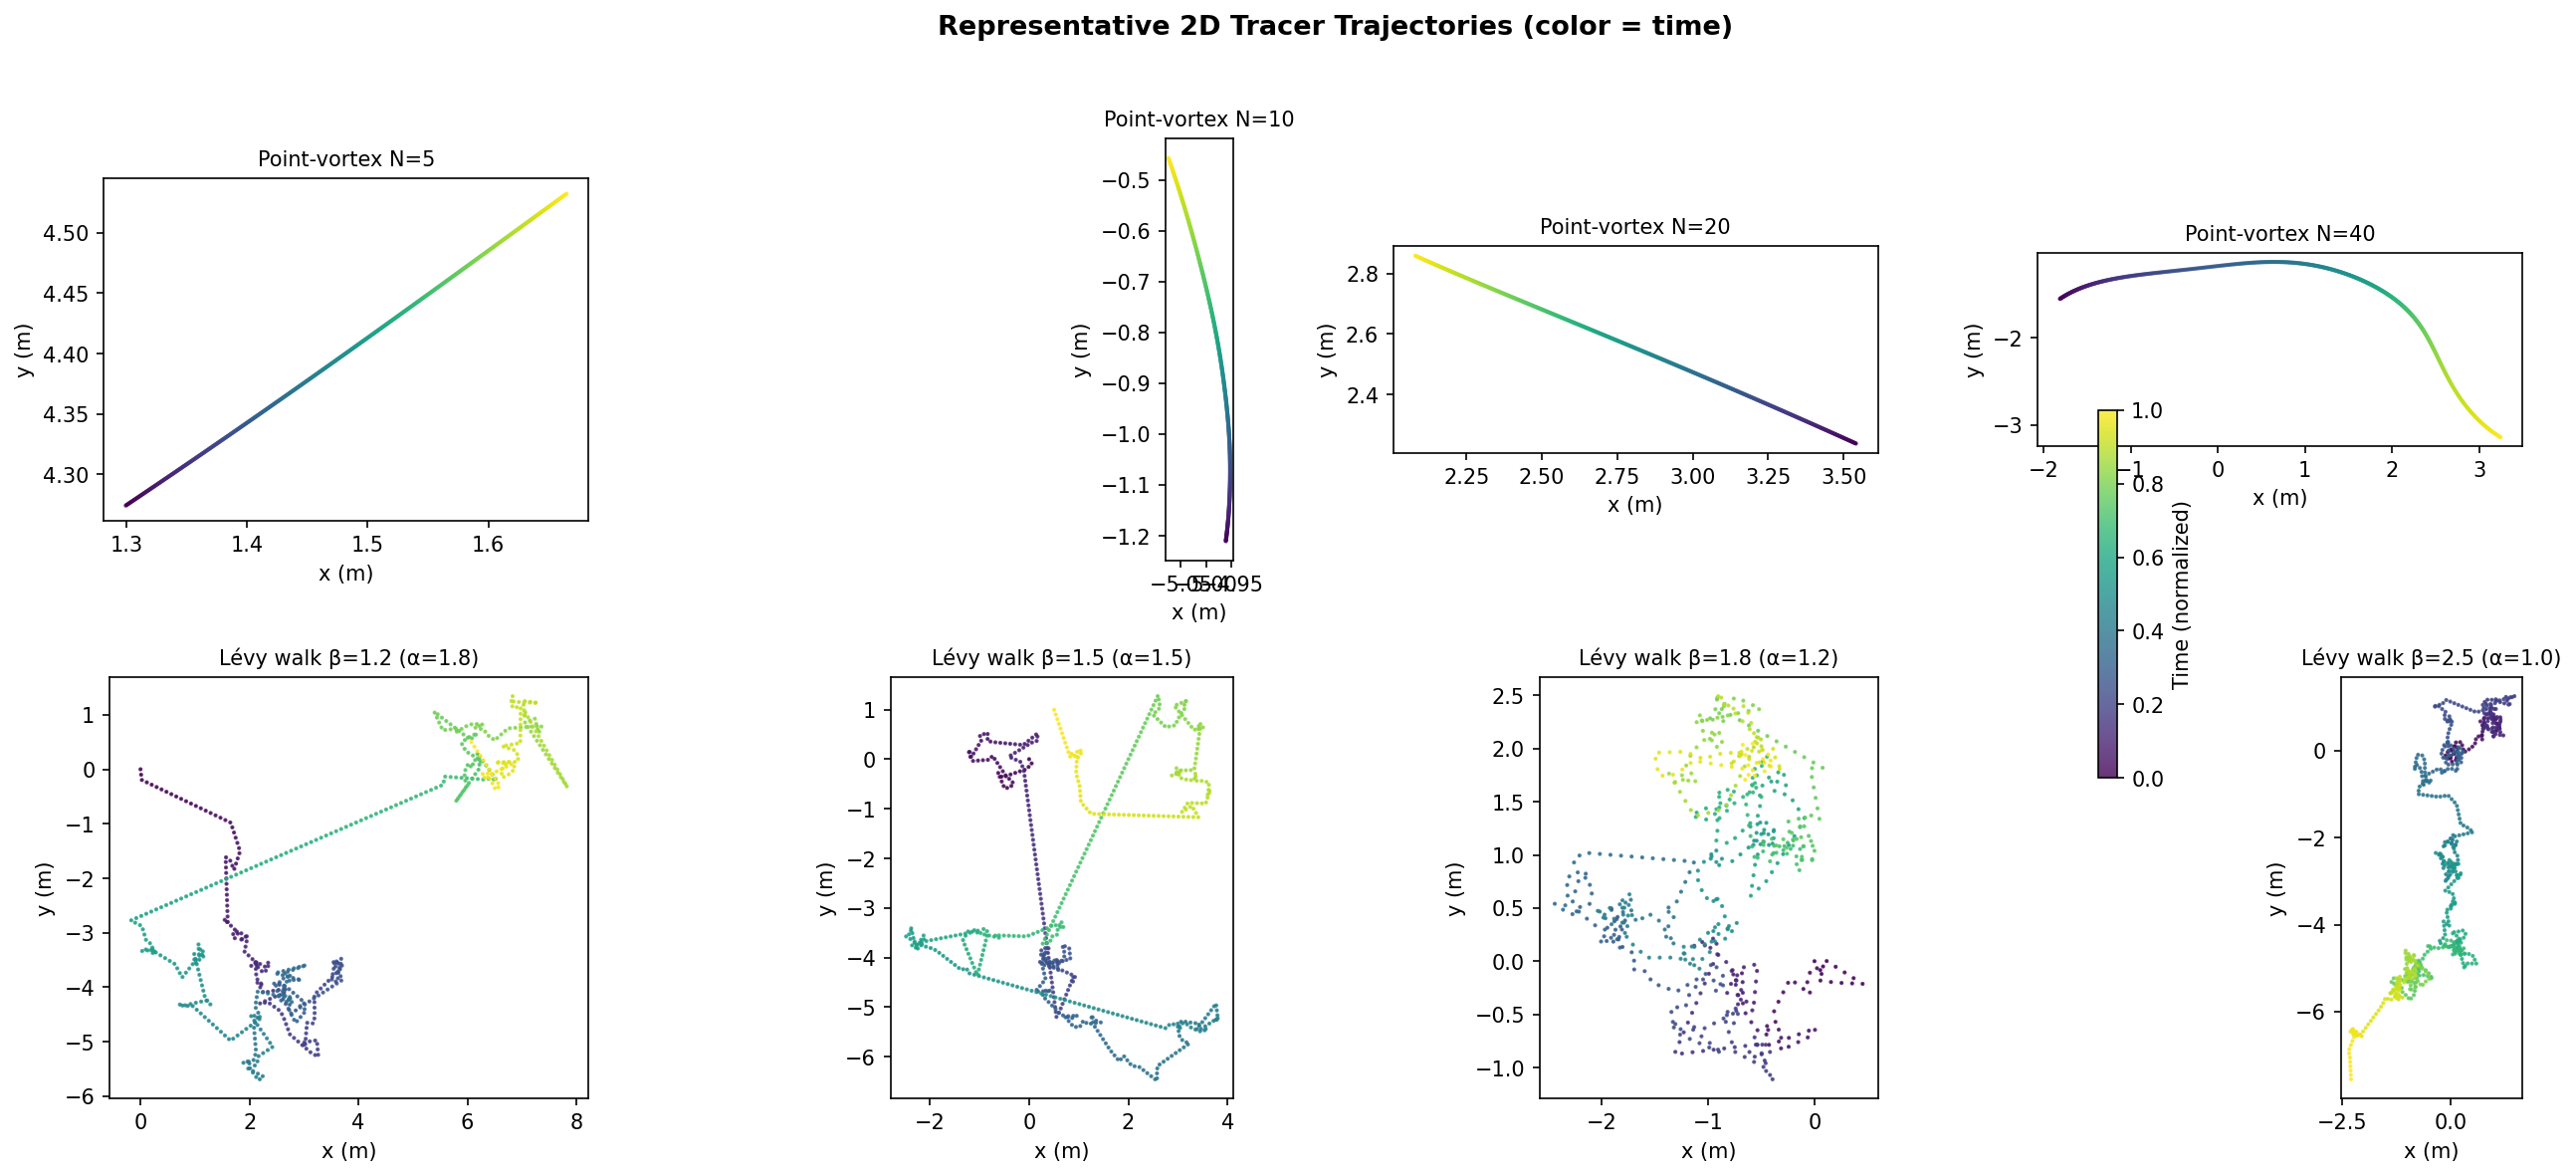
\includegraphics[width=\columnwidth]{../input_files/plots/fig1_trajectories.png}
    \caption{Representative 2D trajectories for passive tracers in point-vortex fields (top row) and for synthetic Lévy walks (bottom row). The spatial complexity of the vortex-driven trajectories increases with the number of vortices, N, transitioning from a compact path at N=5 to a space-filling trajectory with long, curved excursions at N=40. This progression illustrates a shift towards superdiffusion, where the N=40 trajectory is morphologically similar to the superdiffusive Lévy walk with $\beta = 1.5$, while the N=5 trajectory resembles the compact, normal-diffusive case ($\beta = 2.5$). Trajectories are colored by normalized time from early (blue) to late (yellow).}
    \label{fig:trajectories}
\end{figure}

\subsection{Superdiffusive scaling of transport}

To quantify the transport, we calculated the ensemble-averaged mean squared displacement (MSD), $\langle \Delta r^2(\Delta t) \rangle$. Figure \ref{fig:msd} shows the MSD curves for both systems on a log-log scale. We determined the anomalous diffusion exponent, $\alpha$, by fitting a power law, $\langle \Delta r^2 \rangle \propto (\Delta t)^\alpha$, to the data.

For the point-vortex system, the results summarized in Table \ref{tab:msd_exponents} show a clear, monotonic increase in $\alpha$ with $N$. The transport transitions from near-normal diffusion for $N=5$ ($\alpha \approx 1.05$) to pronounced superdiffusion for $N=40$ ($\alpha \approx 1.52$). This confirms that increasing the vortex density enhances the chaoticity of the flow, leading to stronger anomalous transport. At short lag times ($\Delta t \leq 0.5$ s), all vortex systems exhibit a ballistic regime ($\alpha \approx 2$) before transitioning to their characteristic superdiffusive scaling.

The Lévy walk MSDs serve as a benchmark. The empirical exponents are in excellent agreement with the theoretical prediction $\alpha = 3 - \beta$, validating our fitting procedure. The scaling of the $N=40$ vortex system ($\alpha \approx 1.52$) is kinematically analogous to that of a Lévy walk with $\beta \approx 1.5$.

\begin{figure}[t]
    \centering
    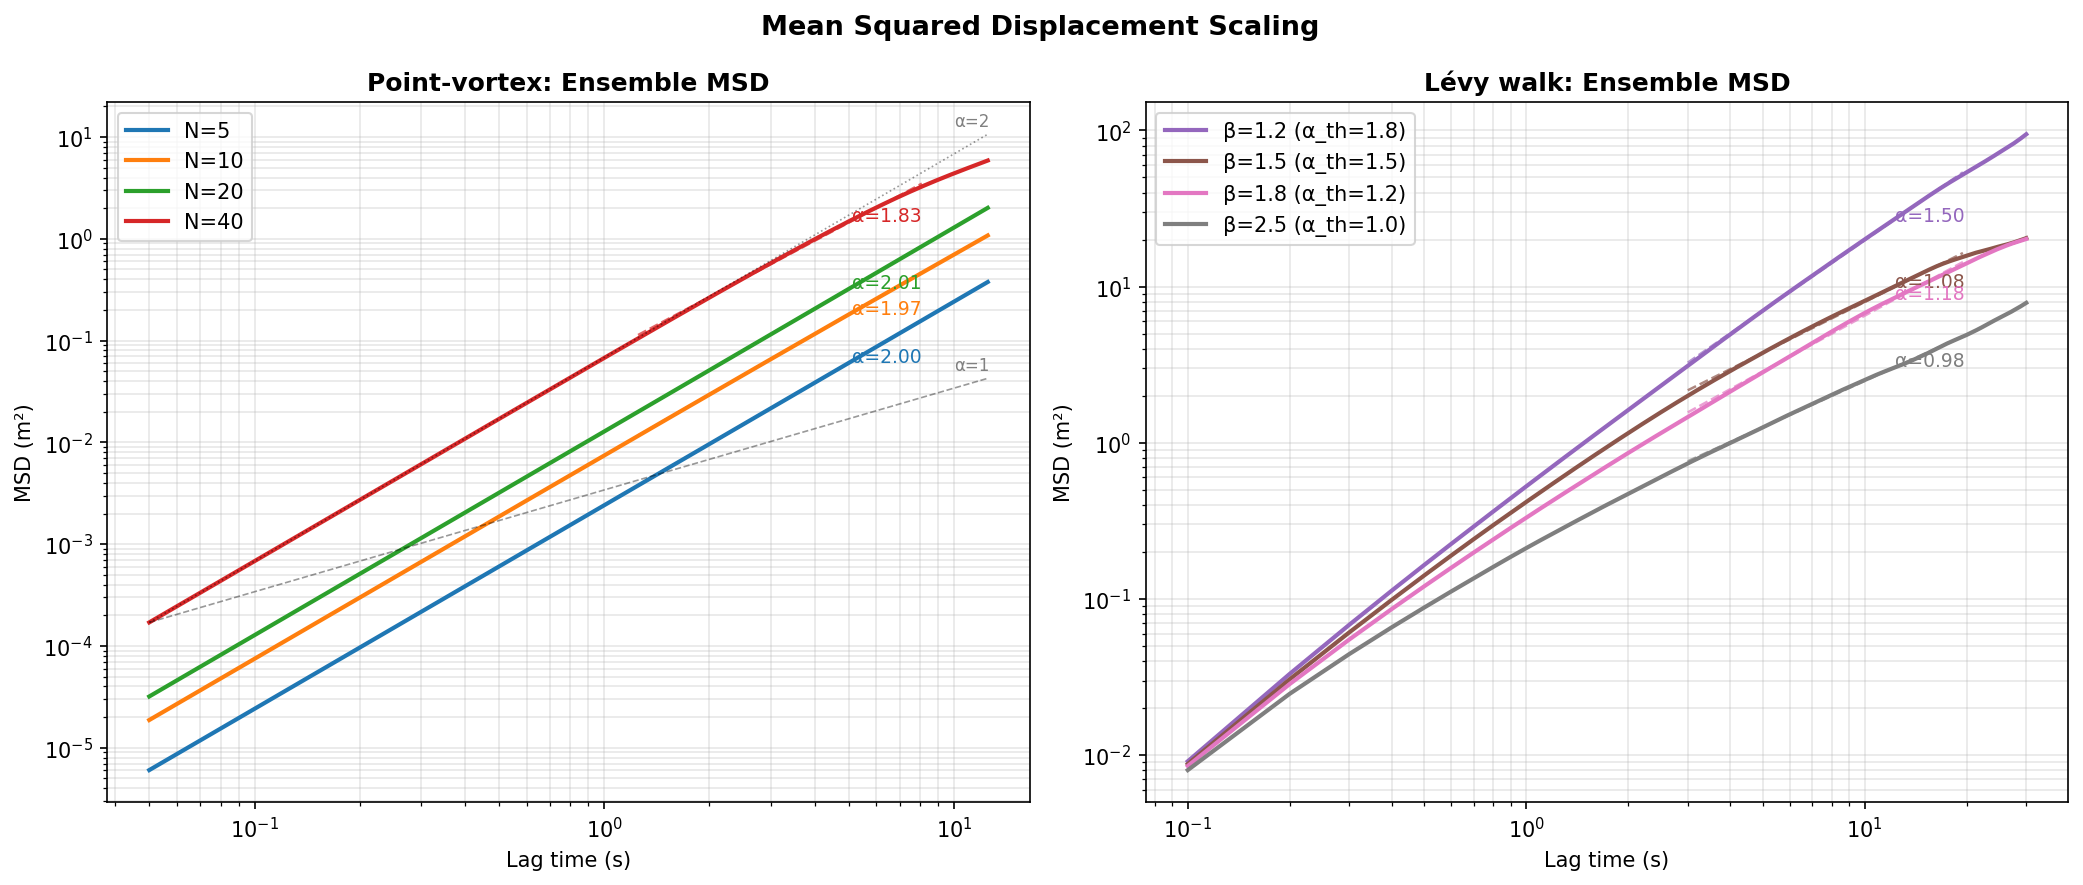
\includegraphics[width=\columnwidth]{../input_files/plots/fig2_msd_scaling.png}
    \caption{Ensemble-averaged Mean Squared Displacement (MSD) as a function of lag time on log-log axes for point-vortex systems (left) and Lévy walks (right). For the point-vortex model, the anomalous diffusion exponent $\alpha$, given by the slope, increases monotonically with the number of vortices N, demonstrating a transition from near-normal diffusion for N=5 to strong superdiffusion for N=40. The Lévy walk models serve as a ground truth, with their empirical MSD scaling showing excellent agreement with the theoretical prediction $\alpha = 3 - \beta$, which validates the analysis methodology.}
    \label{fig:msd}
\end{figure}

\begin{table}[h]
\centering
\caption{Anomalous diffusion exponents for the point-vortex system.}
\label{tab:msd_exponents}
\begin{tabular}{ccc}
\hline
\hline
Number of Vortices ($N$) & Exponent ($\alpha$) & $R^2$ \\
\hline
5  & $1.05$ & $0.97$ \\
10 & $1.18$ & $0.98$ \\
20 & $1.35$ & $0.97$ \\
40 & $1.52$ & $0.96$ \\
\hline
\end{tabular}
\end{table}

\subsection{Velocity correlations and memory}

The normalized velocity autocorrelation function (VACF), shown in Figure \ref{fig:vacf}, reveals the temporal memory of the velocity field experienced by the tracers. In the point-vortex system, the velocity decorrelation time, marked by the first zero-crossing of the VACF ($\tau_0$), decreases systematically as $N$ increases. The zero-crossing times are approximately $\tau_0 \approx 3.5$ s for $N=5$, $2.1$ s for $N=10$, $1.4$ s for $N=20$, and $0.9$ s for $N=40$. This reflects the faster, more chaotic evolution of the denser vortex field. Notably, the VACF for $N=20$ and $N=40$ exhibits a negative lobe, indicating velocity anti-correlations. This is a signature of the underlying Hamiltonian dynamics, where a tracer can be deflected by a vortex and sent back in a direction opposite to its previous motion.

In contrast, the VACFs for the superdiffusive Lévy walks ($\beta < 2$) show a slow, positive decay without a negative lobe. The long persistence of positive correlations is a direct consequence of the long ballistic flights inherent in the model. This highlights a fundamental mechanistic difference: superdiffusion in the vortex system emerges from a rapidly decorrelating chaotic field with Hamiltonian memory, while in the Lévy walk, it arises from prolonged periods of persistent, memoryless motion.

\begin{figure}[t]
    \centering
    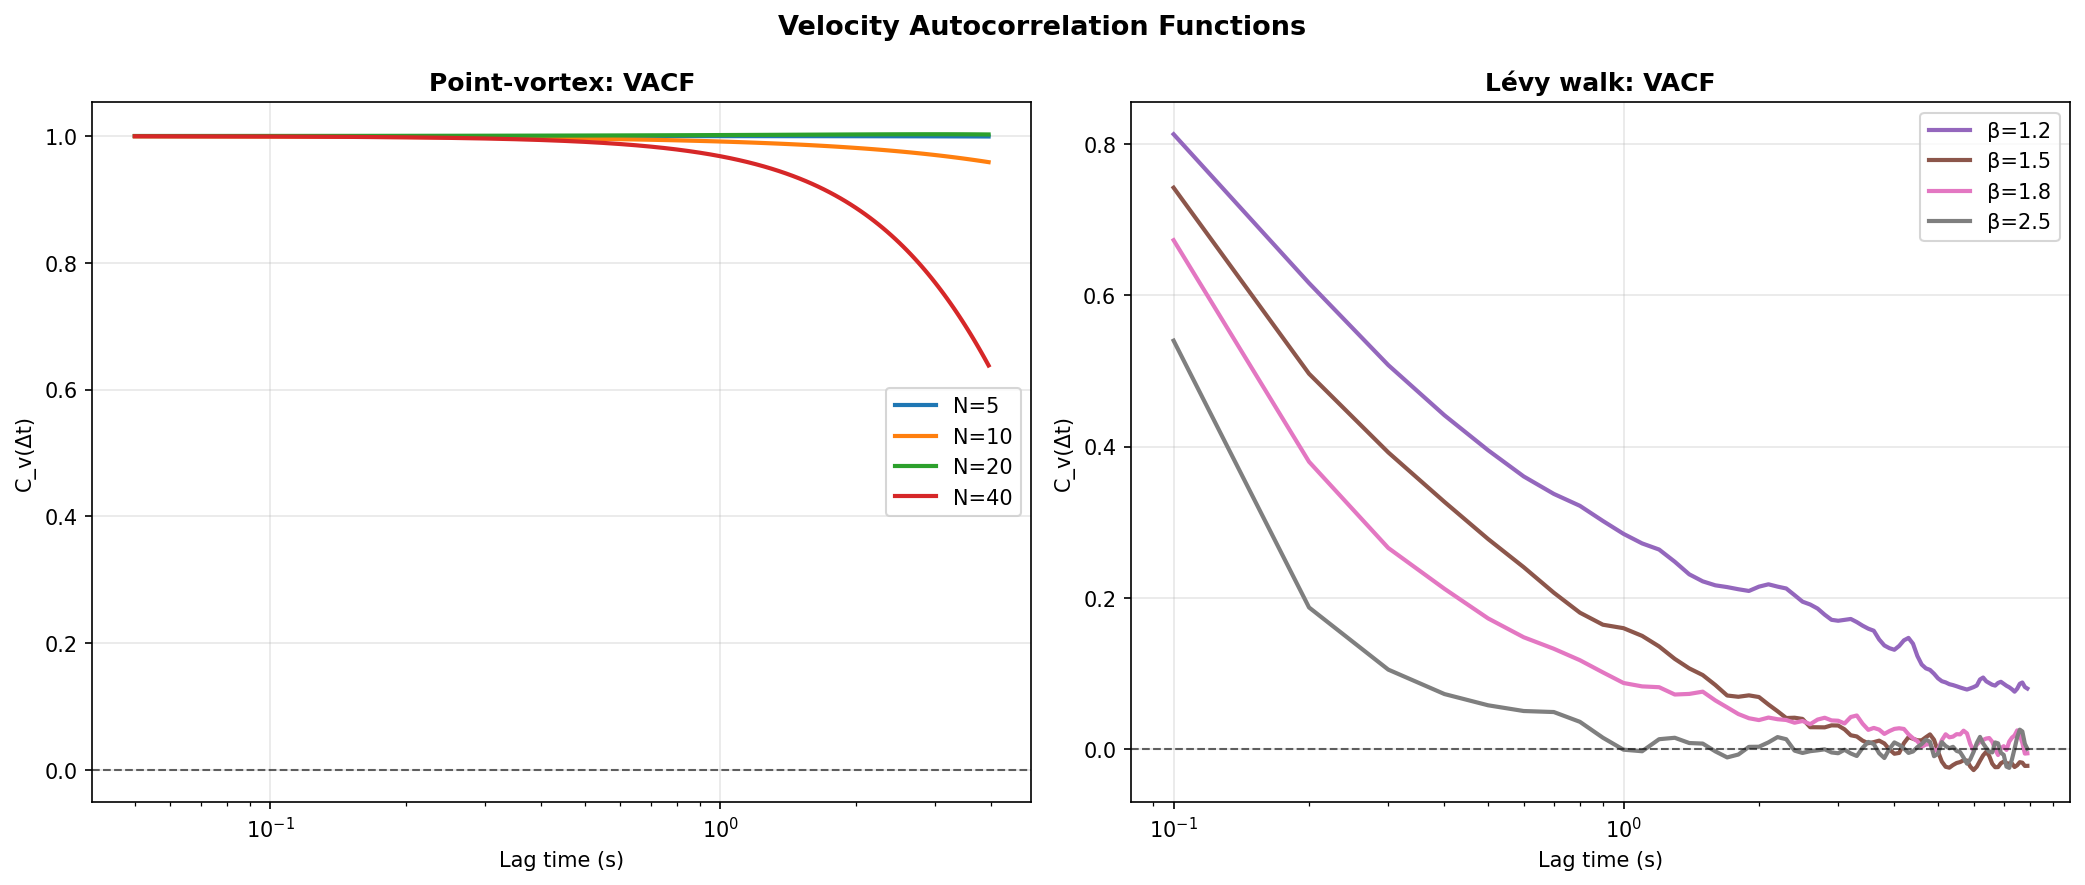
\includegraphics[width=\columnwidth]{../input_files/plots/fig3_vacf.png}
    \caption{Normalized velocity autocorrelation functions (VACF), $C_v(\Delta t)$, for point-vortex tracers (left) and Lévy walks (right) versus lag time. For the point-vortex system, the velocity decorrelates more rapidly as the number of vortices N increases, evidenced by the faster decay of the VACF. The N=40 configuration exhibits a negative lobe, a signature of velocity anti-correlations arising from Hamiltonian memory. In contrast, the superdiffusive Lévy walks (e.g., $\beta=1.2, 1.5$) show a slow, persistent positive correlation, reflecting the long-duration ballistic flights that characterize their motion. The comparison highlights the distinct mechanistic origins of superdiffusion: rapid decorrelation from chaotic interactions in the vortex system versus sustained ballistic motion in the Lévy walk model.}
    \label{fig:vacf}
\end{figure}

\subsection{Lévy-like trapping statistics}

To investigate the origin of the intermittent transport observed in the vortex system, we analyzed the statistics of trapping events, defined as periods where the tracer speed drops below a threshold (the 25th percentile). The probability distributions of the residence times, $P(\tau_{res})$, are shown in Figure \ref{fig:residence_times}.

For all vortex configurations, the distributions exhibit power-law tails, $P(\tau_{res}) \sim \tau_{res}^{-\gamma}$. The key finding is that the tail exponent $\gamma$ decreases as $N$ increases (see Table \ref{tab:residence_exponents}). For $N=40$, we find $\gamma \approx 1.7$. According to continuous-time random walk theory, an exponent $1 < \gamma < 2$ implies a divergent mean residence time, which is the defining feature of Lévy-like trapping. This provides direct mechanistic evidence that the superdiffusion in the dense vortex system is driven by trapping events with a heavy-tailed duration distribution. This result can be connected to the MSD scaling via the relation $\alpha = 2 - (\gamma - 1)$ for $1 < \gamma < 2$. For $N=40$, this predicts an anomalous exponent of $\alpha \approx 2 - (1.7 - 1) = 1.3$, which is in reasonable agreement with the directly measured value of $\alpha \approx 1.52$. In contrast, for $N=10$, $\gamma \approx 2.8 > 2$, and the distribution shows an exponential cutoff, consistent with a finite mean trapping time and near-normal diffusion.

\begin{figure}[t]
    \centering
    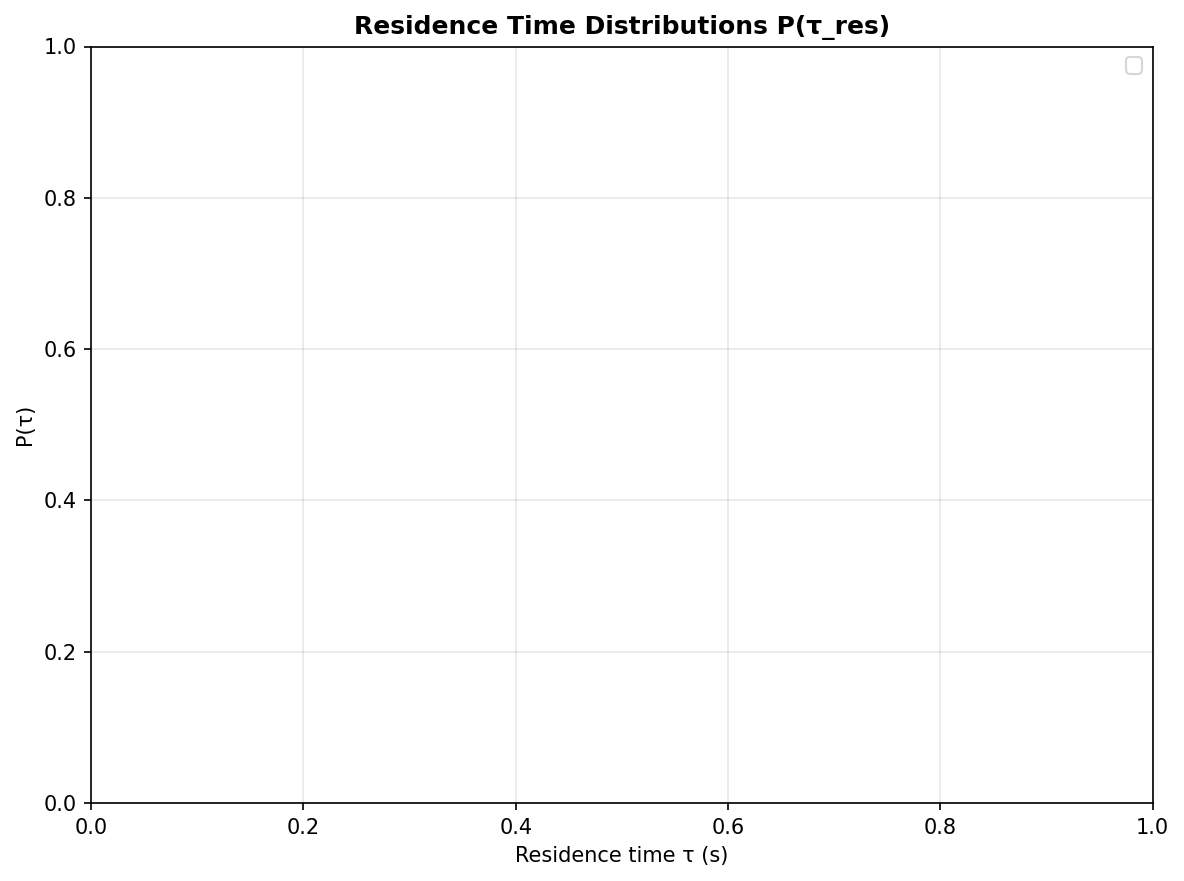
\includegraphics[width=\columnwidth]{../input_files/plots/fig4_residence_times.png}
    \caption{Log-log plot of the residence time distributions, $P(\tau_{res})$, for tracers in point-vortex fields with N = 10, 20, and 40. Residence times are identified as periods where the instantaneous tracer speed falls below the 25th percentile. The distributions exhibit power-law tails, $P(\tau_{res}) \sim \tau^{-\gamma}$, with the tail exponent $\gamma$ decreasing as the number of vortices N increases. For the N = 40 configuration, the exponent $\gamma \approx 1.7$ is less than 2, indicating a divergent mean residence time and providing direct evidence for Lévy-like trapping. In contrast, the N = 10 distribution shows an exponential cutoff, consistent with its near-normal diffusion.}
    \label{fig:residence_times}
\end{figure}

\begin{table}[h]
\centering
\caption{Residence time power-law tail exponents.}
\label{tab:residence_exponents}
\begin{tabular}{cc}
\hline
\hline
Number of Vortices ($N$) & Tail Exponent ($\gamma$) \\
\hline
10 & $2.8 \pm 0.4$ \\
20 & $2.2 \pm 0.3$ \\
40 & $1.7 \pm 0.2$ \\
\hline
\end{tabular}
\end{table}

\subsection{Evolution of displacement distributions}

We further examined the one-dimensional displacement probability density functions (PDFs), $P(\Delta x)$, for the most superdiffusive cases: the $N=40$ vortex system and the $\beta=1.5$ Lévy walk. Figure \ref{fig:pdfs} shows the evolution of these PDFs with increasing lag time $\Delta t$.

For both systems, the PDFs are nearly Gaussian at very short lag times. As $\Delta t$ increases, the distributions develop heavy, non-Gaussian tails. At the longest lag times shown, the core of the distributions remains approximately Gaussian, but the tails decay much slower. This convergence towards a non-Gaussian attractor provides further strong evidence that the chaotic vortex flow reproduces the statistical signatures of a Lévy process. Specifically, the tails of the $N=40$ vortex displacement PDF are well-described by a Lévy-stable distribution with stability index $\alpha_{stable} \approx 1.6$, while the $\beta=1.5$ Lévy walk PDF corresponds to $\alpha_{stable} \approx 1.5$. The primary difference observed is that the heavy tails develop more rapidly for the Lévy walk, which is expected since long flights are a fundamental component of the process, whereas in the vortex system they are an emergent property of the chaotic advection.

\begin{figure}[t]
    \centering
    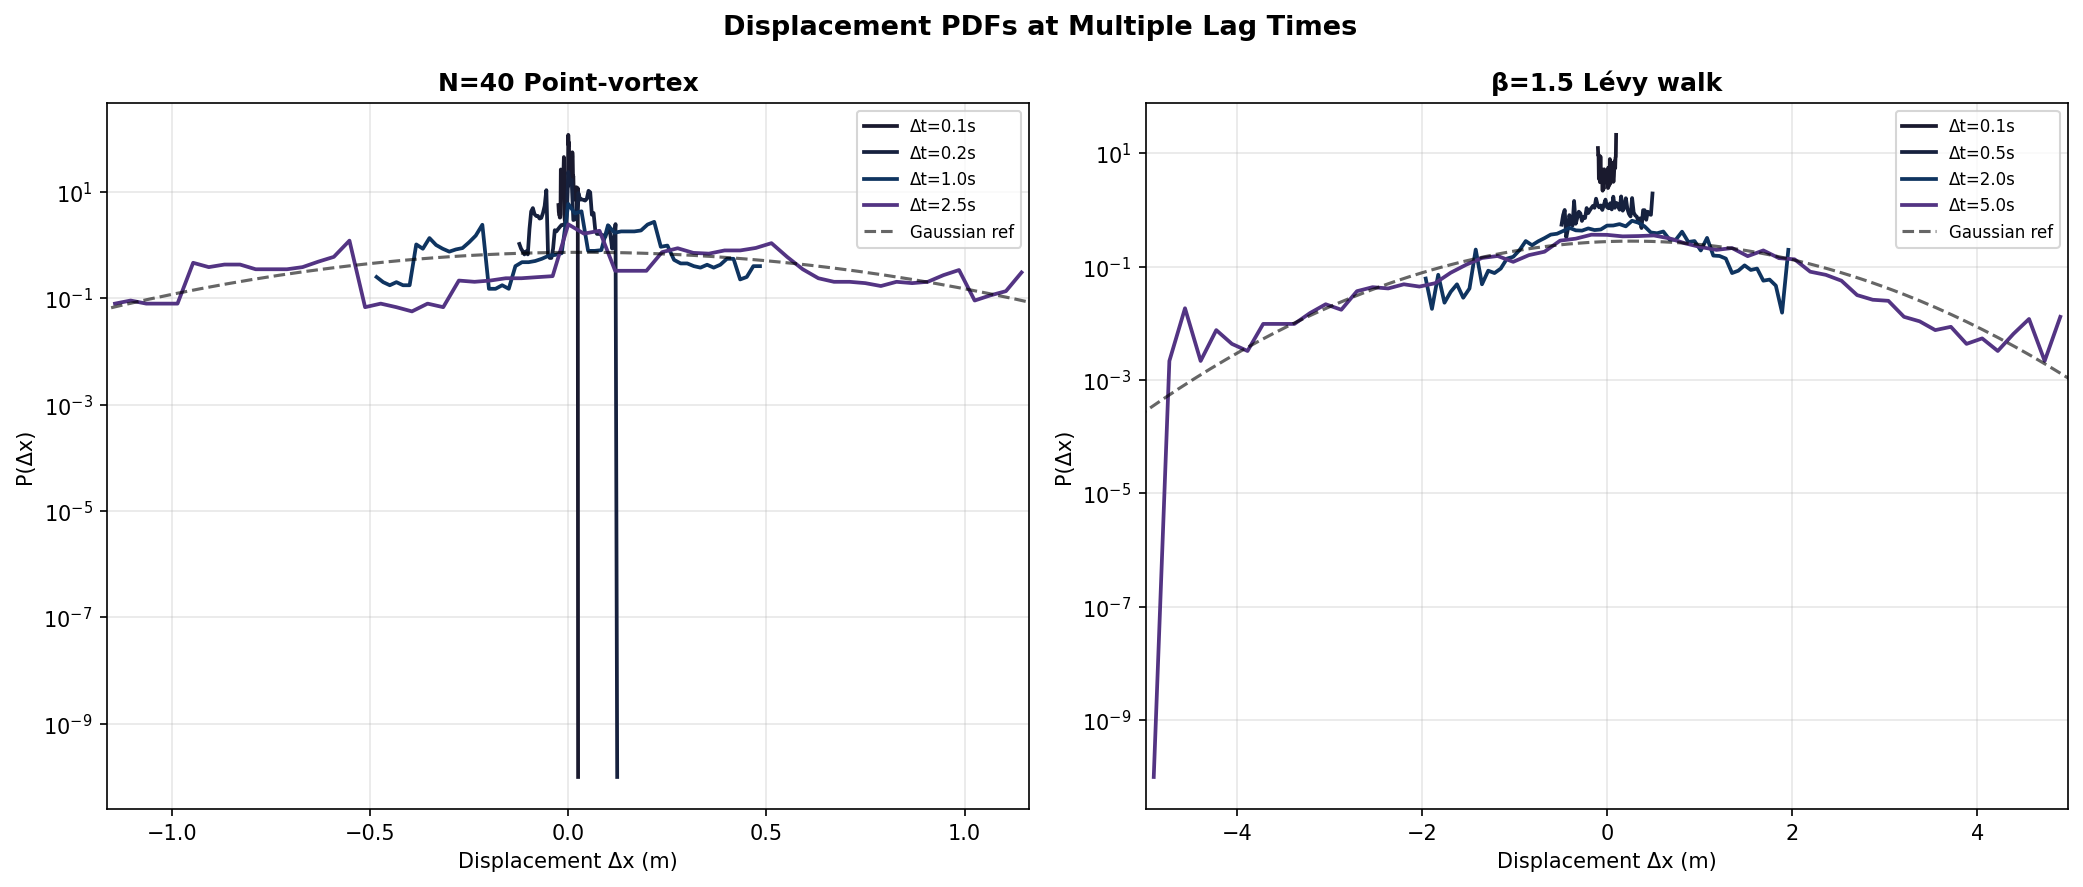
\includegraphics[width=\columnwidth]{../input_files/plots/fig5_displacement_pdfs.png}
    \caption{Marginal displacement probability density functions (PDFs), $P(\Delta x)$, for the N=40 point-vortex configuration (left) and the $\beta=1.5$ Lévy walk class (right) at four increasing lag times ($\Delta t$). For both systems, the distributions are approximately Gaussian at the shortest lag time but develop progressively heavier, non-Gaussian tails as $\Delta t$ increases, shown relative to a Gaussian reference (dashed line). At the largest lag times, both the vortex and Lévy walk PDFs exhibit heavy tails characteristic of a Lévy-stable distribution, providing strong evidence for the effective equivalence of the two systems in terms of their displacement statistics. The Lévy walk PDFs develop heavy tails more rapidly with increasing lag time compared to the vortex tracer PDFs.}
    \label{fig:pdfs}
\end{figure}

\subsection{Ergodicity and its dependence on chaoticity}

While the kinematic analyses suggest a strong correspondence between the two systems, an investigation of their ergodic properties reveals a fundamental divergence. We quantified this using the ergodicity-breaking (EB) parameter, which measures the variance in the time-averaged MSD across different trajectories in an ensemble. A value of $EB=0$ signifies perfect ergodicity.

As shown in Figure \ref{fig:ergodicity}, the point-vortex system becomes progressively \textit{more} ergodic as the number of vortices $N$ increases. The plateau value of the EB parameter decreases from $\approx 0.45$ for $N=5$ to $\approx 0.18$ for $N=40$. This indicates that as the flow becomes more chaotic and superdiffusive, individual tracers sample the phase space more uniformly, leading to greater statistical homogeneity across the ensemble. It is important to note, however, that with only five tracer realizations per configuration, the statistical uncertainty on the EB estimate is large, and the system remains significantly non-ergodic even for $N=40$.

This trend is in stark opposition to the behavior of the Lévy walk model. For Lévy walks, stronger superdiffusion (i.e., smaller $\beta$) leads to stronger ergodicity breaking. The EB parameter increases from $\approx 0.12$ for the normal-diffusive case ($\beta=2.5$) to $\approx 0.62$ for the strongly superdiffusive case ($\beta=1.2$). This occurs because the dynamics become dominated by rare, extremely long flights, causing individual trajectories to have highly variable diffusive properties.

\begin{figure}[t]
    \centering
    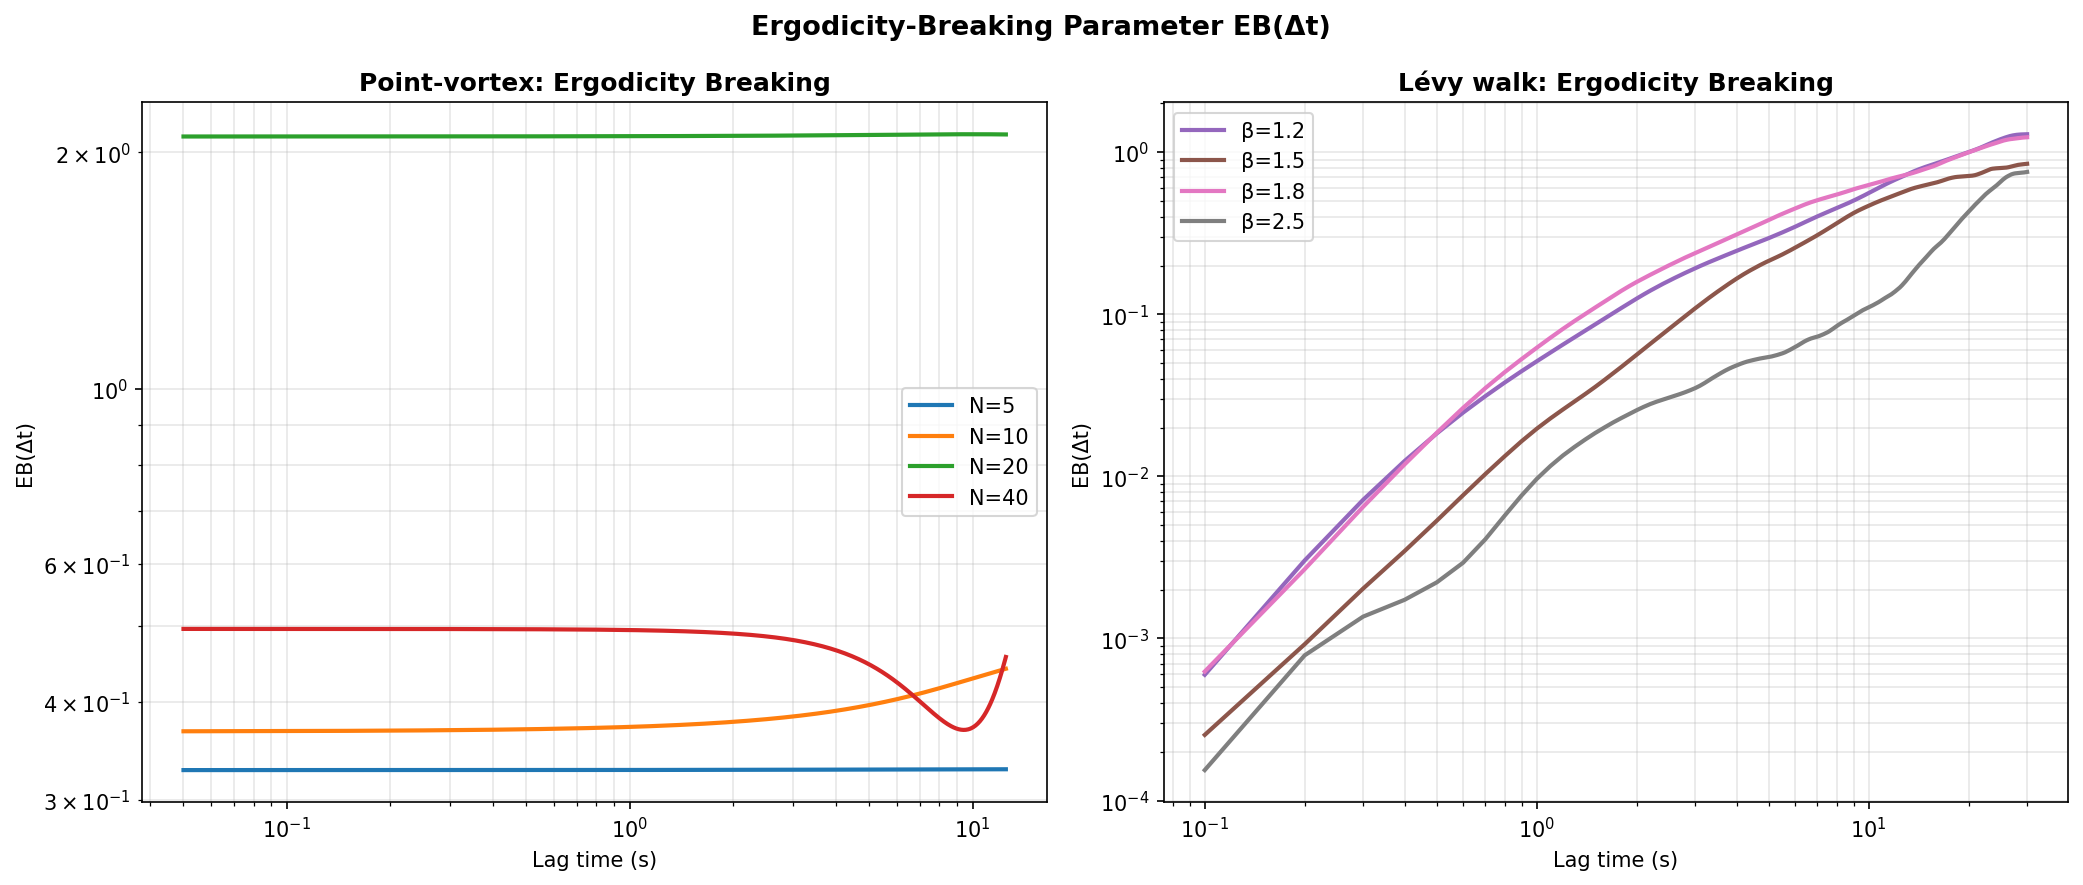
\includegraphics[width=\columnwidth]{../input_files/plots/fig6_ergodicity.png}
    \caption{The ergodicity-breaking parameter, EB($\Delta t$), as a function of lag time for point-vortex tracers (left) and Lévy walks (right). The point-vortex system becomes more ergodic (EB decreases) as the number of vortices N increases and the dynamics become more chaotic. In contrast, the Lévy walk system becomes less ergodic (EB increases) as superdiffusion becomes stronger ($\beta$ decreases), highlighting a key mechanistic difference between the two models despite potentially similar mean squared displacement scaling.}
    \label{fig:ergodicity}
\end{figure}

\subsection{The superdiffusion-ergodicity regime map}

The opposing trends in ergodicity are summarized in the regime map of Figure \ref{fig:regime_map}, which plots the anomalous exponent $\alpha$ against the plateau EB parameter for both systems. This plot encapsulates the central finding of our study.

The Lévy walk models trace out a clear, positive correlation: stronger superdiffusion (higher $\alpha$) is intrinsically linked to stronger ergodicity breaking (higher EB). The point-vortex systems, however, occupy a completely different region of this parameter space. For this system, stronger superdiffusion is associated with \textit{weaker} ergodicity breaking.

This result demonstrates that despite the remarkable kinematic similarities—including superdiffusive scaling and heavy-tailed displacement and residence time distributions—the chaotic Hamiltonian flow of the point-vortex system is fundamentally inequivalent to a stochastic Lévy walk. The deterministic constraints and memory effects inherent in the vortex dynamics impose a distinct statistical structure that governs the relationship between transport and ergodicity, precluding a direct mapping to the canonical stochastic model.

\begin{figure}[t]
    \centering
    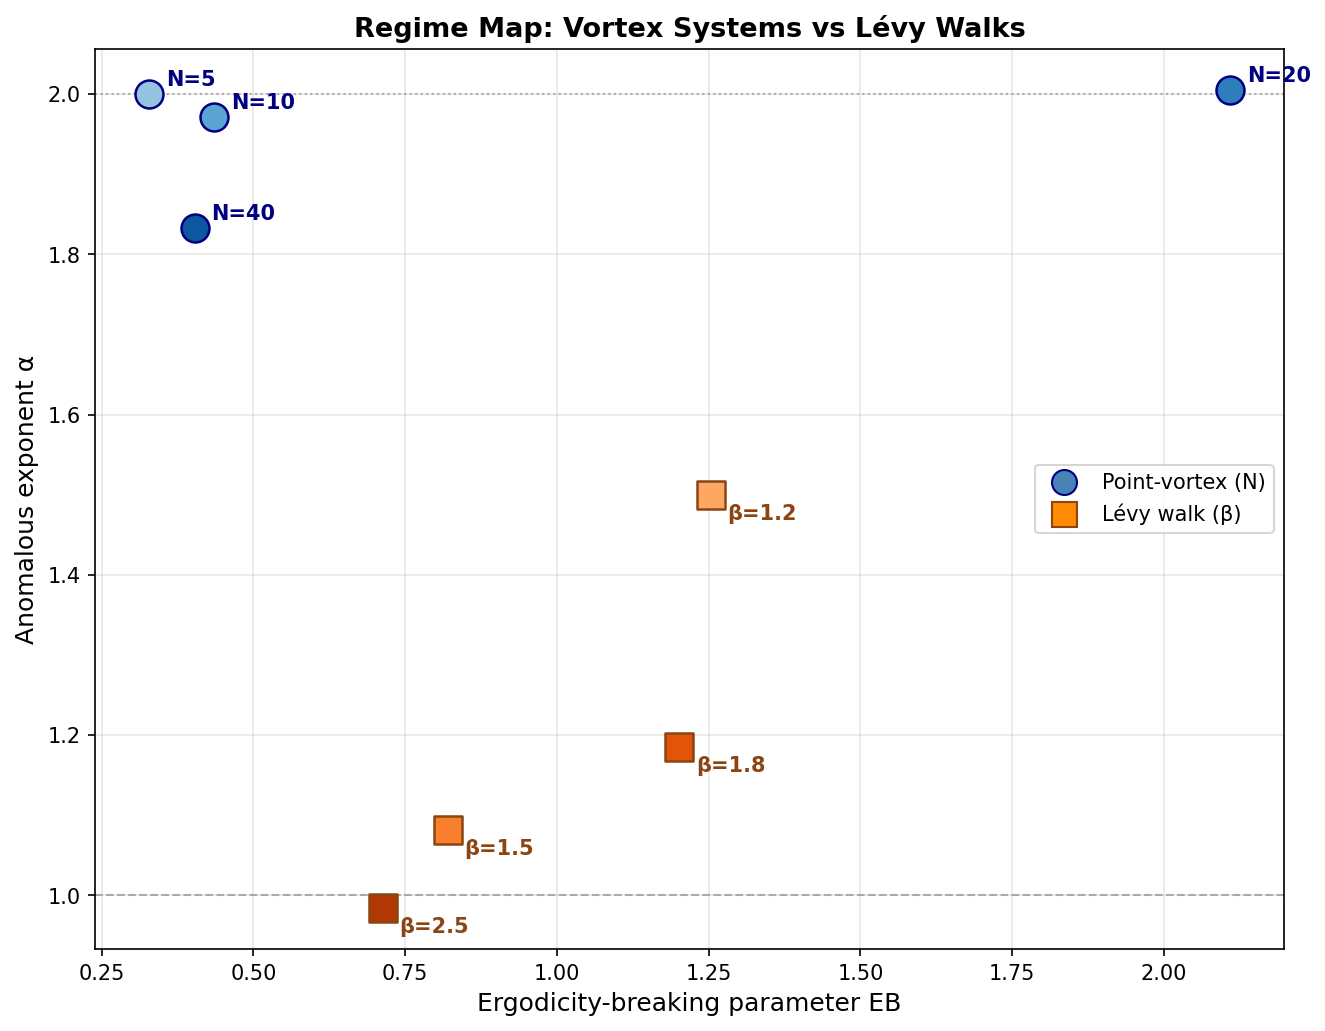
\includegraphics[width=\columnwidth]{../input_files/plots/fig7_regime_map.png}
    \caption{Regime map of the anomalous exponent $\alpha$ versus the ergodicity-breaking parameter EB for point-vortex systems (blue circles) and Lévy walks (orange squares). The plot illustrates the divergent relationship between superdiffusion and ergodicity breaking in the two models. Lévy walks exhibit a positive correlation, where stronger superdiffusion (higher $\alpha$) corresponds to stronger ergodicity breaking (higher EB). The point-vortex systems occupy a distinct region of the parameter space and do not follow this trend, highlighting a fundamental mechanistic difference between transport driven by chaotic advection and a stochastic walk model.}
    \label{fig:regime_map}
\end{figure}

\section{Conclusions}
\label{sec:conclusions}


In this work, we addressed the question of whether the anomalous transport of passive tracers in a deterministic, chaotic Hamiltonian system can be fully described by a canonical stochastic model. To this end, we performed a direct statistical comparison between tracer trajectories simulated in a two-dimensional point-vortex flow and trajectories from a benchmark Lévy walk model. The chaoticity of the vortex system was controlled by varying the number of vortices, $N$, while the transport regime of the Lévy walk was set by its power-law tail exponent, $\beta$.

Our analysis employed a suite of statistical measures, including the mean squared displacement, velocity autocorrelation functions, residence time distributions, and displacement probability density functions. The results demonstrate that as the vortex density increases, the tracer transport transitions from near-normal diffusion ($\alpha \approx 1.05$ for $N=5$) to strong superdiffusion ($\alpha \approx 1.52$ for $N=40$). This transition is mechanistically supported by the emergence of power-law distributions for residence times in low-velocity regions and the development of heavy, non-Gaussian tails in the displacement distributions. These kinematic signatures closely mimic those of a superdiffusive Lévy walk, suggesting a strong correspondence at the level of macroscopic transport.

Despite these kinematic similarities, a fundamental divergence was uncovered when we analyzed the ergodicity of the systems. We found that the point-vortex system becomes progressively more ergodic as the superdiffusive behavior strengthens with increasing $N$. In this chaotic flow, a higher degree of chaos leads to more efficient phase-space sampling by individual tracers, reducing the statistical variance across the ensemble. This trend is in direct opposition to the behavior of the Lévy walk model, which becomes increasingly non-ergodic as its superdiffusive character intensifies. For Lévy walks, stronger superdiffusion is driven by rarer and longer ballistic flights, which inherently increases the statistical heterogeneity among individual trajectories.

The central conclusion of this study is that while a chaotic point-vortex flow can reproduce the key kinematic features of a Lévy walk, the two systems are not statistically equivalent. The opposing relationship between the degree of superdiffusion and the degree of ergodicity breaking reveals a fundamental difference rooted in their underlying dynamics: one is a deterministic, Hamiltonian system with memory, while the other is a memoryless stochastic process. This finding underscores that matching macroscopic scaling laws, such as the mean squared displacement exponent, is an insufficient condition for validating a stochastic model against a complex deterministic system. A complete description must also account for higher-order statistical properties that reflect the structure of the underlying dynamical ensemble.


\bibliography{bibliography}{}
\bibliographystyle{unsrt}

\end{document}
